	\graphicspath{{../suyluancungbi/sudoku2/}}
	\vskip 0.2cm
	\textit{\textbf{\color{toancuabi}Bi tiếp tục giới thiệu cùng bạn đọc phiên bản “nguyên thủy” của trò chơi Sudoku, đó là Sudoku phiên bản số. Phiên bản này thích hợp cho các bé từ $7$ tuổi trở lên.
	Ở phiên bản số, người ta không chỉ quan tâm đến các số trong mỗi hàng, mỗi cột, mà còn quan tâm đến các số trong mỗi “vùng”.}}
	\begin{multicols}{2}
		Ở Hình $12$ là một bảng $4\times4$ và bốn bảng con $2\times2$ được phân chia ra từ bảng $4\times4$ đó, mỗi bảng con được tô bởi một màu. \textit{Ở các bài $1, 2, 4, 5$ dưới đây, mỗi bảng con $2\times2$ như thế được gọi là một vùng}.
		\begin{figure}[H]
			\centering
			\vspace*{5pt}
			\captionsetup{labelformat= empty, justification=centering}
			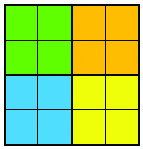
\includegraphics[scale=0.8]{pic1}
			\caption{\small\textit{Hình $12.$}}
			\vspace*{-10pt}
		\end{figure}
	\end{multicols}
	\vspace*{-5pt}
	Giờ, các bé hãy cùng Bi vượt qua thử thách đầu tiên với Sudoku  số nhé!
	\vskip 0.1cm
	\textbf{\color{toancuabi}Ví dụ $\pmb{3.}$} Điền các số $1, 2, 3, 4$ vào các ô vuông còn trống trong bảng ở Hình $13$, sao cho trong mỗi hàng, mỗi cột và trong mỗi vùng, mỗi số chỉ xuất hiện một lần.
	\vskip 0.1cm
	\begin{wrapfigure}{l}{0.35\textwidth}
		\centering
%		\vspace*{5pt}
		\captionsetup{labelformat= empty, justification=centering}
		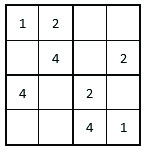
\includegraphics[scale=0.8]{pic2}
		\caption{\small\textit{Hình $13.$}}
		\vspace*{-10pt}
	\end{wrapfigure}
	\textbf{\color{toancuabi}\textit{Cùng Bi suy luận:}}
	\vskip 0.1cm
	-- Rõ ràng, với mỗi ô còn trống, chúng mình sẽ phải cân nhắc các khả năng điền, rồi lựa chọn số thích hợp để điền. Vì thế, chúng mình nên bắt đầu từ những ô mà số khả năng điền phải cân nhắc là ít hơn cả, các bé nhỉ? Từ điều kiện
	“trong mỗi hàng, mỗi cột và trong mỗi vùng, mỗi số chỉ xuất hiện một lần”, hiển nhiên suy ra trong mỗi hàng, cũng như mỗi cột, hay mỗi vùng, phải có đủ cả bốn số $1$, $2$, $3$, $4$. Như thế, trong mỗi hàng, mỗi cột, mỗi vùng, số nằm ở ô này sẽ “áp đặt” số nằm ở ô kia. Do đó, ô trống nằm ở hàng hay cột hay vùng nào đã có nhiều số được điền sẽ “bị” nhiều “áp đặt” hơn cả, và vì thế, sẽ có số khả năng điền cần cân nhắc ít hơn cả, phải không các bé?
	\vskip 0.1cm
	\begin{multicols}{2}
		-- Nhìn bảng ở Hình $13$, chúng mình thấy, có hai vùng, mà mỗi vùng đều đã có ba số được điền (nói cách khác, đều chỉ có một ô trống): vùng trên bên trái và vùng dưới bên phải (xem Hình $14$). Với những suy luận vừa nêu trên, chắc chắn chúng mình phải bắt đầu từ những ô trống ở hai vùng đó rồi!
		\begin{figure}[H]
			\centering
			\vspace*{-10pt}
			\captionsetup{labelformat= empty, justification=centering}
			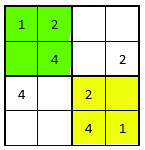
\includegraphics[scale=0.8]{pic3}
			\caption{\small\textit{Hình $14.$}}
%			\vspace*{-5pt}
		\end{figure}
	\end{multicols}
	\vspace*{-5pt}
		-- Cùng xem nào! Ở mỗi vùng, trong hai vùng được tô màu ở Hình $14$, đều đã có ba số $1$, $2$, $4$, vậy thì ở ô trống của mỗi vùng đó chắc chắn phải là số $3$ rồi! Chúng mình cùng điền số $3$ vào ô trống ở mỗi vùng đó nhé (xem Hình $15$).
		\vskip 0.1cm
		\begin{wrapfigure}{l}{0.47\textwidth}
			\centering
%			\vspace*{5pt}
			\captionsetup{labelformat= empty, justification=centering}
			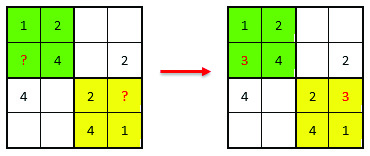
\includegraphics[width=0.48\textwidth]{pic4}
			\caption{\small\textit{Hình $15.$}}
			
			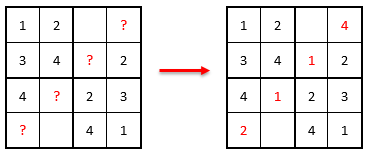
\includegraphics[width=0.48\textwidth]{pic5}
			\caption{\small\textit{Hình $16.$}}
			\vspace*{-10pt}
		\end{wrapfigure}
	-- Trong bảng nhận được ở Hình $15$ không còn có những vùng, mà ở đó đã có ba số được điền. Tuy nhiên, như các bé thấy đấy, lại có những cột, những hàng, mà ở mỗi cột hay hàng đó đều đã có ba số được điền; đó là các cột thứ $1$, thứ $4$ (tính từ trái qua phải), và các hàng thứ $2$, thứ $3$ (tính từ trên xuống dưới). Vì thế, nhờ điều kiện “ở mỗi hàng, mỗi cột phái có đủ cả bốn số $1, 2, 3, 4$”, chúng mình sẽ tìm ra được số cần điền vào ô tróng ở mỗi hàng, mỗi cột ấy, phải không nào? Chẳng hạn, xét cột thứ $1$. Vì trong cột đã có ba số $1, 3, 4$ nên số cần điền vào ô trống ở cột đó bắt buộc phải là $2$ rồi. Tương tự như thế cho việc tìm ra các số cần điền vào ô trống ở cột thứ $4$, cũng như ở hàng thứ $2$, và hàng thứ $3$. Chúng mình cùng điền nhé (xem Hình $16$).
	\vskip 0.1cm
	\begin{wrapfigure}{r}{0.3\linewidth}
		\centering
		\vspace*{-5pt}
		\captionsetup{labelformat= empty, justification=centering}
		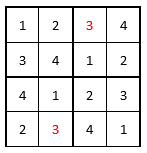
\includegraphics[scale=0.8]{pic6}
		\caption{\small\textit{Hình $17.$}}
		\vspace*{-15pt}
	\end{wrapfigure}
	-- Tiếp theo, bằng cách suy luận tương tự trên, chắc hẳn các bé sẽ tìm ra ngay được hai số cần điền vào hai ô trống trong bảng nhận được ở Hình $5$ nhỉ? Các bé hãy tự mình hoàn thành việc điền số, rồi so với “đáp số” dưới đây để kiểm tra nhé (xem Hình $17$).
	\vskip 0.1cm
	Giờ hãy cùng Bi thử sức với một sudoku  khác nha!
	\vskip 0.1cm
		\textbf{\color{toancuabi}Ví dụ $\pmb{4.}$} Điền các số $1, 2, 3, 4$ vào các ô vuông còn trống trong bảng ở Hình $18$, sao cho trong mỗi hàng, mỗi cột và trong mỗi vùng, mỗi số chỉ xuất hiện một lần.
		\vskip 0.1cm
		\begin{wrapfigure}{l}{0.3\textwidth}
			\centering
			\vspace*{-18pt}
			\captionsetup{labelformat= empty, justification=centering}
			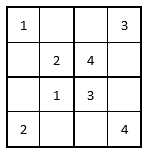
\includegraphics[scale=0.8]{pic7}
			\caption{\small\textit{Hình $18.$}}
			\vspace*{-20pt}
		\end{wrapfigure}
	\textbf{\color{toancuabi}\textit{Lời giải:}}
	\vskip 0.1cm
	-- Quan sát bảng ở Hình $18$, chúng mình không thấy một vùng hay một hàng, một cột nào, mà ở đó đã có ba số được điền. Ở vùng nào, hàng nào, cột nào cũng chỉ có đúng hai số được điền mà thôi. Thế nghĩa là, tình huống ở bài này không tương tự như tình huống ở Ví dụ $3$ rồi! Phải làm sao bây giờ?
	\vskip 0.2cm
	-- Suy đi, tính lại, Bi thấy không còn cách nào khác, ngoài cách chọn một ô trống nào đó, rồi cân nhắc các khả năng điền có thể. Chẳng hạn, ta chọn ô trống có dấu “?” (dưới đây, gọi tắt là ô “?”) trong bảng bên trái, ở Hình $19$. Vì trong mỗi hàng, mỗi cột, mỗi vùng, mỗi số chỉ được có mặt một lần, nên do nằm ở hàng thứ $1$, số ở ô “?” phải khác $1$, $3$; và đồng thời, do nằm ở cột thứ $2$, số đó phải khác $2$, $1$. Do đó, số ở ô “?” phải khác đồng thời cả $1$, $2$ và $3$; vì thế, số đó bắt buộc phải là $4$ (xem Hình $19$).
	\vskip 0.1cm
		\begin{wrapfigure}{l}{0.48\textwidth}
			\centering
			\vspace*{-15pt}
			\captionsetup{labelformat= empty, justification=centering}
			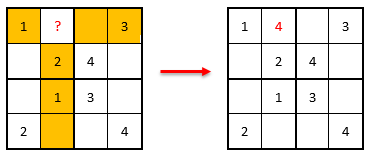
\includegraphics[width=0.47\textwidth]{pic8}
			\vspace*{-5pt}
			\caption{\small\textit{Hình $19.$}}
			\vspace*{-25pt}
		\end{wrapfigure}
	-- Ở bảng nhận được sau bước điền trên đã có những vùng, hàng, cột, mà ở mỗi vùng, hàng, cột đó có ba số được điền. Vì thế, bằng các suy luận tương tự như khi giải Ví dụ $3$, chúng mình đã có thể tiếp tục điền các số thích hợp vào các ô trống còn lại rồi. Các bé tự làm tiếp nhé.
	\vskip 0.1cm
	\begin{wrapfigure}{r}{0.3\textwidth}
		\centering
		\vspace*{-30pt}
		\captionsetup{labelformat= empty, justification=centering}
		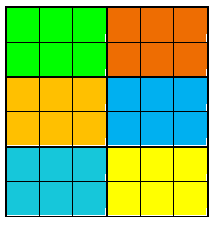
\includegraphics[scale=0.5]{pic9}
		\vspace*{-5pt}
		\caption{\small\textit{Hình $20.$}}
		\vspace*{-25pt}
	\end{wrapfigure}
		Ở Hình $20$ là một bảng $6\times6$ và sáu bảng con $2\times3$ được phân chia ra từ bảng $6\times6$ đó, mỗi bảng con được tô bởi một màu. Ở các bài $3$, $6$ dưới đây, mỗi bảng con $2\times3$ như thế cũng được gọi là một vùng.
		\vskip 0.1cm
		\begin{wrapfigure}{r}{0.3\textwidth}
			\centering
			\vspace*{-25pt}
			\captionsetup{labelformat= empty, justification=centering}
			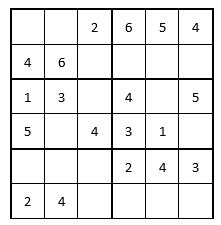
\includegraphics[scale=0.5]{pic10}
			\vspace*{-5pt}
			\caption{\small\textit{Hình $21.$}}
			\vspace*{-20pt}
		\end{wrapfigure}
	\textbf{\color{toancuabi}Ví dụ $\pmb{5.}$} Điền các số $1$, $2$, $3$, $4$, $5$, $6$ vào các ô vuông còn trống trong bảng ở Hình $21$, sao cho trong mỗi hàng, mỗi cột và trong mỗi vùng, mỗi số chỉ xuất hiện một lần.
	\vskip 0.1cm
	\textbf{\color{toancuabi}\textit{Cùng Bi suy luận:}}
	\vskip 0.05cm
	-- Quan sát bảng ở Hình $21$, ta thấy không có hàng, cột hay vùng nào, mà ở đó đã có năm số được điền, để từ đó suy ra ngay số ở ô trống phải là số nào. Vì thế, tương tự như việc giải Ví dụ $4$, điều cần làm trước hết là chọn ra ô trống đầu tiên để điền số.
	\vskip 0.05cm
	\begin{wrapfigure}{r}{0.3\textwidth}
		\centering
		\vspace*{-15pt}
		\captionsetup{labelformat= empty, justification=centering}
		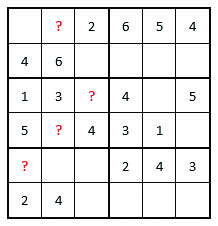
\includegraphics[scale=0.5]{pic11}
		\vspace*{-5pt}
		\caption{\small\textit{Hình $22.$}}
		\vspace*{-15pt}
	\end{wrapfigure}
	-- Như đã nêu ở trên, ta cần chọn ra ô trống mà số được điền ở ô đó chịu nhiều “áp đặt” hơn cả, từ các số đã có ở trong hàng, trong cột, trong vùng có chứa ô ấy. Quan sát kỹ bảng ở Hình $21$, Bi thấy có bốn ô trống có tính chất như vậy; đó là các ô “?” trong bảng ở Hình $22$.
	\vskip 0.1cm
	Mỗi ô “?” trong bảng trên đều chịu năm “áp đặt” khác nhau. Vì thế, chúng mình có thể chọn một ô tùy ý trong các ô đó, đề bắt đầu thực hiện việc điền số. Ta chọn ô “?” nằm ở giao của hàng thứ $3$ và cột thứ $3$, các bé nhé. Vì ô này nằm ở hàng thứ $3$, và ở hàng đó đã có các số $1, 3, 4, 5$, nên số ở ô đó phải khác $1, 3, 4, 5$ (trong mỗi hàng, mỗi số chỉ được có mặt một lần mà). Đồng thời, do ô đang xét nằm ở cột thứ $3$, và ở cột này đã có các số $2, 4$, nên số ở ô đó phải khác $2, 4$ (đố các bé biết vì sao?). Từ đó suy ra, số được điền vào ô đang xét phải khác $1, 2, 3, 4$ và $5$; vì thế, số ấy bắt buộc phải là $6$ (xem Hình $23$).
	\begin{figure}[H]
		\centering
		\vspace*{-10pt}
		\captionsetup{labelformat= empty, justification=centering}
		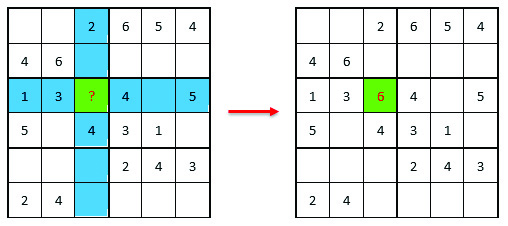
\includegraphics[width=0.48\textwidth]{pic12}
		\caption{\small\textit{Hình $24.$}}
		\vspace*{-15pt}
	\end{figure}
	-- Xét tương tự trên đối với các ô “?” còn lại, ta sẽ tìm được các số cần điền vào các ô đó (xem Hình $24$).
	\begin{multicols}{2}
		\begin{figure}[H]
			\centering
			\vspace*{-5pt}
			\captionsetup{labelformat= empty, justification=centering}
			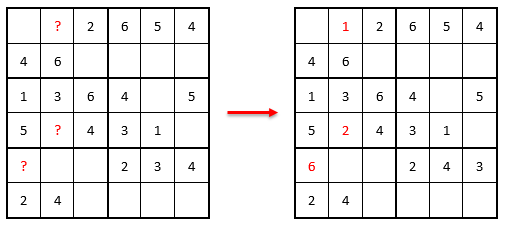
\includegraphics[width=0.48\textwidth]{pic13}
			\caption{\small\textit{Hình $24.$}}
			\vspace*{-10pt}
		\end{figure}
		\begin{figure}[H]
			\centering
			\vspace*{-5pt}
			\captionsetup{labelformat= empty, justification=centering}
			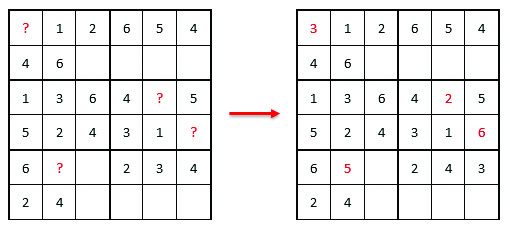
\includegraphics[width=0.48\textwidth]{pic14}
			\caption{\small\textit{Hình $25.$}}
			\vspace*{-10pt}
		\end{figure}
	\end{multicols}
	-- Trong bảng mới nhận được ở Hình $24$, đã có những hàng, những cột, mà trong mỗi hàng, mỗi cột ấy đều có năm ô đã được điền số; đó là, các hàng thứ $1$, thứ $3$, thứ $4$, và cột thứ $2$. Rõ ràng, với những hàng, những cột này, ta sẽ xác định được ngay số cần điền vào ô trống ở mỗi hàng, mỗi cột ấy (xem Hình $25$).
	\vskip 0.1cm
	-- Quan sát bảng mới nhận được ở Hình $25$, ta thấy có thể xác định được số cần điền vào các ô “?” trong bảng ở Hình $26$ dưới đây.
	\vskip 0.1cm
		\begin{wrapfigure}{l}{0.25\textwidth}
		\centering
		\vspace*{-15pt}
		\captionsetup{labelformat= empty, justification=centering}
		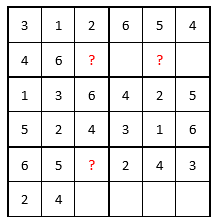
\includegraphics[scale=0.48]{pic15}
		\vspace*{-5pt}
		\caption{\small\textit{Hình $26.$}}
		\vspace*{-15pt}
	\end{wrapfigure}
	Cụ thể, căn cứ các số đã được điền trong hàng thứ $2$ và cột thứ $5$, ta sẽ xác định được số cần điền vào ô “?” nằm ở giao của hàng và cột đó; căn cứ các số đã được điền trong vùng trên cùng  bên trái, ta sẽ xác định được số cần điền vào ô “?” nằm ở giao của hàng thứ $2$ và cột thứ $3$; căn cứ các số đã được điền trong hàng thứ $5$, ta sẽ xác định được số cần điền vào ô “?” nằm ở hàng đó (xem Hình $27$).
	\begin{figure}[H]
		\centering
		\vspace*{-10pt}
		\captionsetup{labelformat= empty, justification=centering}
		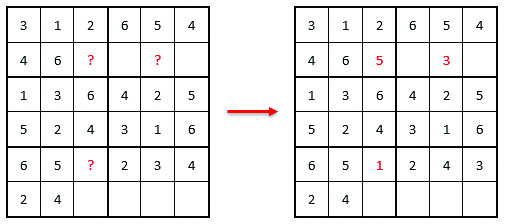
\includegraphics[width=0.48\textwidth]{pic16}
		\vspace*{-5pt}
		\caption{\small\textit{Hình $27$}}
		\vspace*{-10pt}
	\end{figure}
	-- Bằng cách áp dụng các suy luận tương tự trên, ta có các bước điền số tiếp theo, được thể hiện trong Hình $28$ dưới đây.
	\begin{figure}[H]
		\centering
		\vspace*{-10pt}
		\captionsetup{labelformat= empty, justification=centering}
		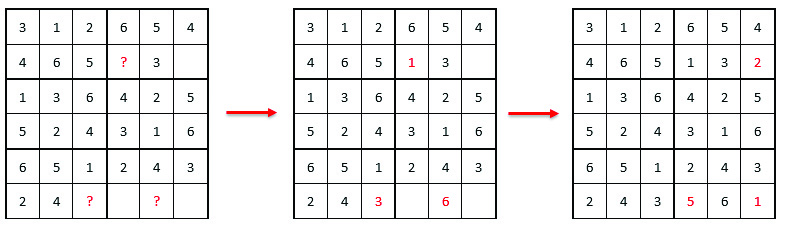
\includegraphics[width=0.8\textwidth]{pic17}
		\vspace*{-5pt}
		\caption{\small\textit{Hình $28.$}}
		\vspace*{-5pt}
	\end{figure}
	Sau đây là một số thử thách sudoku dành cho các bé. Bi chúc các bé có những giờ phút thư giãn vui vẻ và trải nghiệm thật nhiều cảm xúc với trò chơi này nhé!
	\vskip 0.15cm
	\textbf{\color{toancuabi}Bài tập $\pmb{5}$.} Điền các số $1, 2, 3, 4$ vào các ô vuông còn trống trong bảng ở Hình $29$, sao cho trong mỗi hàng, mỗi cột và trong mỗi vùng, mỗi số chỉ xuất hiện một lần.
	\begin{multicols}{3}
		\begin{figure}[H]
			\centering
			\vspace*{-5pt}
			\captionsetup{labelformat= empty, justification=centering}
			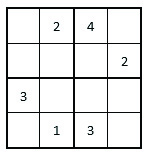
\includegraphics[height=0.22\textwidth]{pic18}
			\caption{\small\textit{Hình $29.$}}
			\vspace*{-10pt}
		\end{figure}
		\begin{figure}[H]
			\centering
			\vspace*{-5pt}
			\captionsetup{labelformat= empty, justification=centering}
			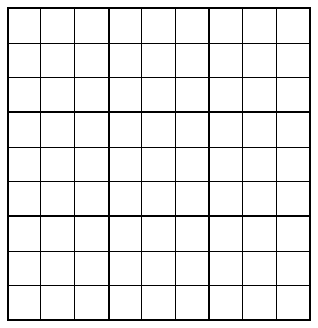
\includegraphics[height=0.22\textwidth]{pic21}
			\caption{\small\textit{Hình $30.$}}
			\vspace*{-10pt}
		\end{figure}
		\begin{figure}[H]
			\centering
			\vspace*{-5pt}
			\captionsetup{labelformat= empty, justification=centering}
			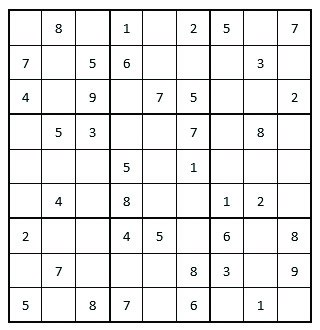
\includegraphics[height=0.22\textwidth]{pic22}
			\caption{\small\textit{ Hình $31.$}}
			\vspace*{-10pt}
		\end{figure}
	\end{multicols}
	\textbf{\color{toancuabi}Bài tập $\pmb{6}$.} Bảng $9\times9$ được phân chia thành chín bảng con $3\times3$ (xem Hình $30$); dưới đây, ta gọi mỗi bảng con $3\times3$ trong phân chia đó là  một vùng.
	\vskip 0.1cm
	Điền các số $1, 2, 3, 4, 5, 6, 7, 8, 9$ vào các ô vuông còn trống trong bảng ở Hình $31$, sao cho trong mỗi hàng, mỗi cột và trong mỗi vùng, mỗi số chỉ xuất hiện một lần.